\autsection{General Approach}{Nelián Colón}

Due to the nature of project, most of the work will be completed trough
developer workstations. At first, the team will be developing different parts of
the system as they are all loosely coupled. Test driven development will be
done, meaning that after each part gets successfully developed and unit tested,
only then they are integrated and tested from a bigger perspective. The project
is divided into 4 major parts, these are: front end client, back end server,
test framework, and repository manager, as shown in Figure~\ref{arqu}. The team
will be using a single cloud hosted Git repository (GitHub) where the project's
code will live, and will follow best revision control practices. Moreover, the
team will follow the Scrum agile development process and will confine to good
planning and documentation.

\begin{figure}[H]
	\centering
	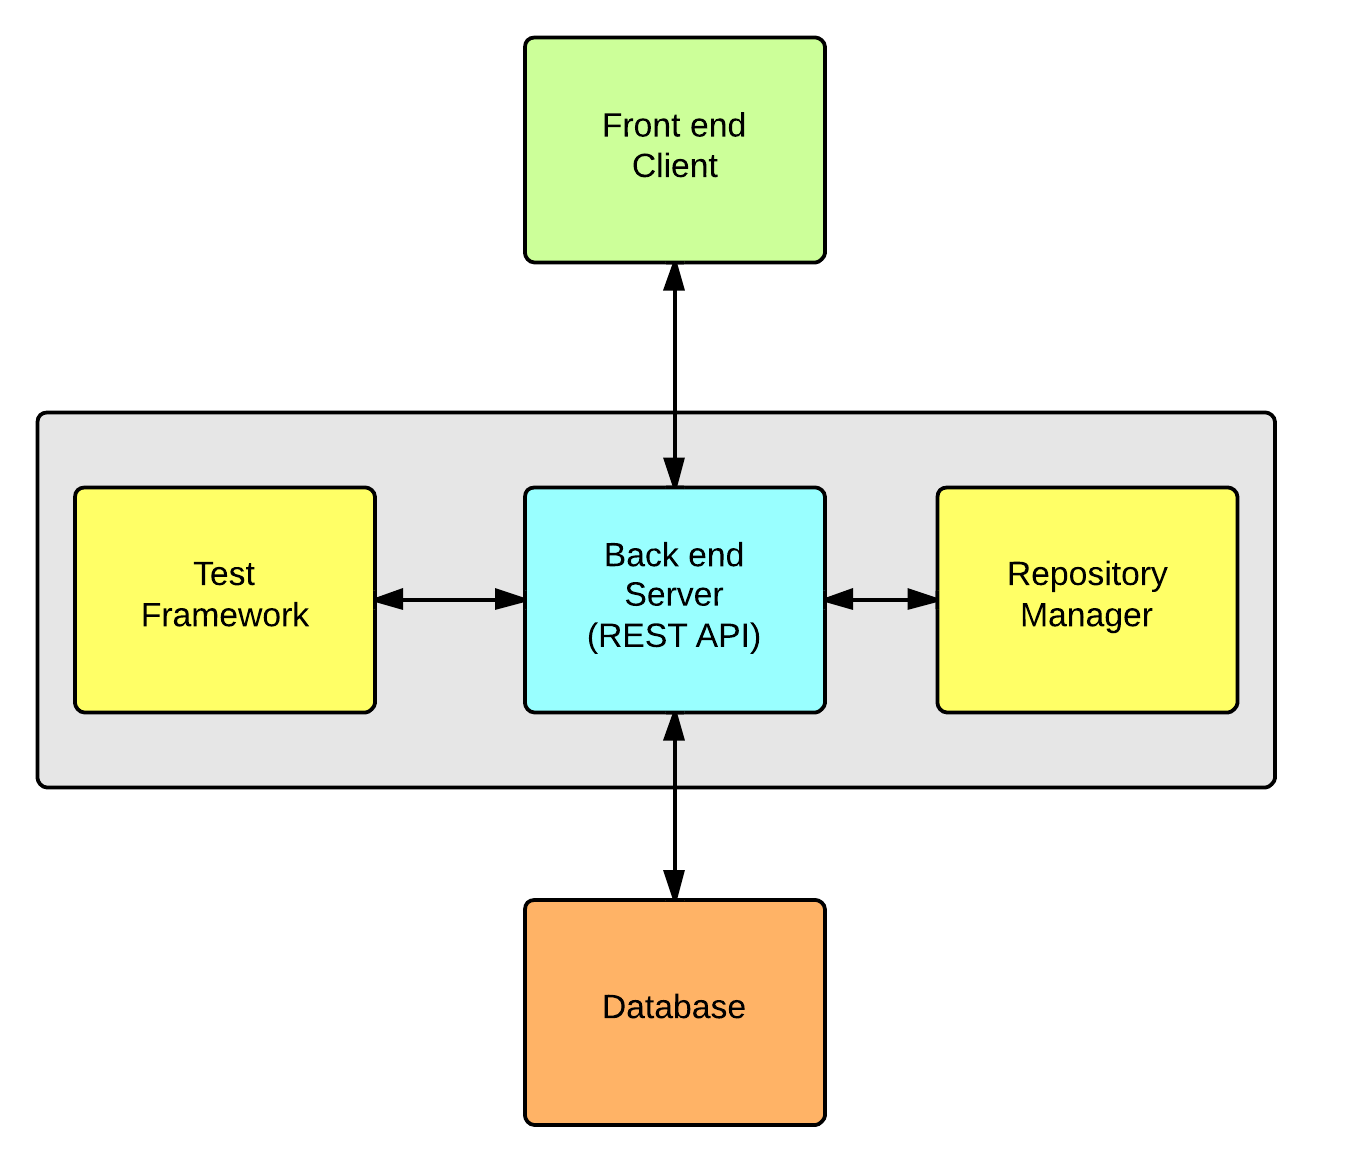
\includegraphics[width=\textwidth]{img/bigArquitectOverview}
	\caption{General overview of the system\label{arqu}}
\end{figure}

\subsection{Meetings and Work Hours}

Team Aguacate will hold weekly meetings on Tuesdays from 3:00 pm to 4:00 pm to
discuss progress and project details. During the meetings, each team member will
state his or her progress, any needs he orshe might have and whether their
schedule has changed. Work hours on assigned tasks will occur every Monday,
Wednesday, and Friday from 9:30 am to 11:20 am unless there is a seminar
scheduled for that day. Other work hours will be every possible day from 6:00 pm
to 9:00 pm minimum. The team will work on sprints, so a sprint planning meeting
will occur on Thursdays from 3:00 pm to 4:00 pm whenever a new sprint comes.
Meeting agenda minutes will be posted in the project blog:
\url{http://pandacodereview.wordpress.com/}.

\subsection{Team Management}

The meetings will be held as described above and other meetings will be
scheduled whenever they are needed. One of the purposes of these meetings is to
make sure that each team member is aware of the other members' progress and
concerns. Changes to these hours are to be discussed and decisions will depend
on majority vote and the project manager's opinion. Each task will have a leader
and an assistant. The leader of each task is completely responsible for the task
and the assistant will assist whenever the leader gets stuck on a problem.
Whenever a conflict arises, the members involved are responsible for finding a
mediator as soon as possible to help them solve the problem.

\subsection{Documentation Standards}
See Appendix~\ref{sec:stand} to see documentation standards.